% !TeX root = ../../main.tex
% Add the above to each chapter to make compiling the PDF easier in some editors.

\chapter{Background and Foundations}\label{chapter:Background and Foundations}

This chapter represents the basic concepts used throughout our work. First, a brief introduction to the reinforcement learning field. Second, Markov Decision Processes (MDPs), the standard mathematical formalism framework for reinforcement learning will be introduced. Then, We will discuss the Value functions and Policy Gradient with the focus on Q-Learning. Next, we will discuss the methods used and differentiate between them. After that, we conclude with the use of deep learning with reinforcement learning with some of Deep Reinforcement Learning Algorithms. Finally, we discuss the challenges and limitation in Reinforcement Learning field.

\section{Reinforcement Learning}
Reinforcement Learning \textbf{RL} (\textit{The science of decision making}) is a machine learning approach to teach agent how to solve tasks through trial and error interaction with a dynamic, unknown environment. Where it formalizes the idea that \textit{\textbf{rewarding or punishing}} an agent for its behavior makes it more likely to repeat or forego that behavior in the future. In contrast with other machine learning methods, the agent is not told the proper actions to take. Instead, the agent interacts with its environment and, upon observing the consequences of its actions, can learn to alter its own behavior in response to rewards received. The goal of the agent is to maximize the expected cumulative reward. The main characters of RL are the \textbf{Agent}\ref{Agent} and the \textbf{Environment}\ref{Environment}. 
% The environment is the world where the agent lives and interacts with. for every interaction, the agent observes the state of the world and based on that takes an action. The environment changes accordingly to the agent's actions and it might also change on its own. 
The typical interaction loop between agent and environment is illustrated in Figure\ref{fig:agent_env}

\begin{figure}[H]
		\begin{center}
				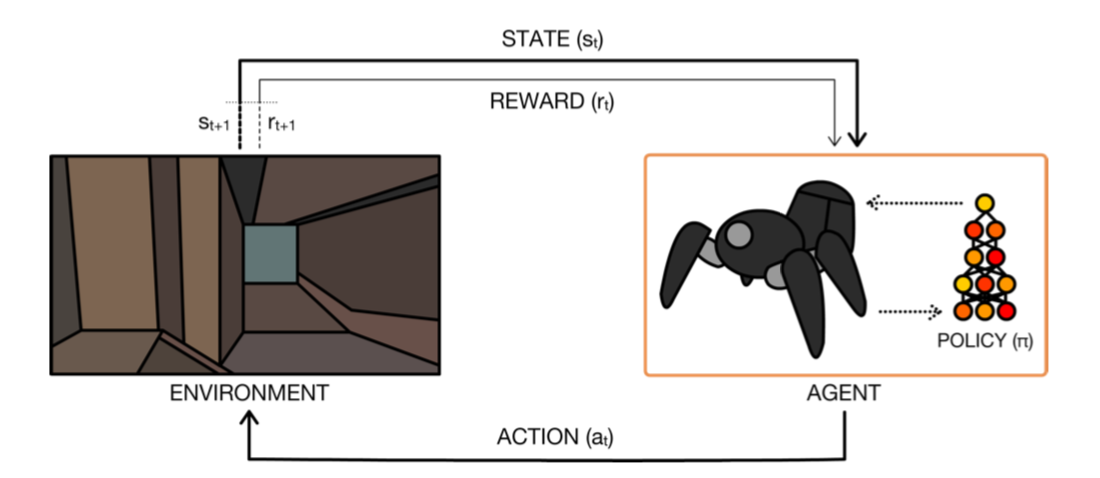
\includegraphics[width=.5\linewidth]{figures/Agent-Env.png}
				\caption{Reinforcement Learning interaction loop. The agent takes an action at a\textsubscript{t} state s\textsubscript{t}. The environment then responds with the corresponding reward r\textsubscript{t+1} and the new state s\textsubscript{t+1}, which are fed back to the agent~\parencite{arulkumaran2017brief}}
				% \caption{Reinforcement Learning interaction loop. [\citetitle{sutton2018reinforcement}]}
				\label{fig:agent_env}
		\end{center}
\end{figure}

\subsection{Agent}\label{Agent}
An agent is the brain who decides to takes proper actions and it's where the learning process happen and improve over time. Examples of the agents, a drone making a delivery, a robot learning to walk or Super Mario navigating a video game. The RL algorithm is the agent, and in life, the agent is you (human being). 
for the learning process, the agent observes the state of the world and based on that takes an action. The environment changes accordingly to the agent's actions and it might also change on its own. 


\subsection{Environment}\label{Environment}
An Environment constitutes a world for the agent to act and learn from. 
To illustrate and describe the environment to an agent we have a \textbf{state} \(s\) which is a complete description of the state of the world, and sometimes An \textbf{observation} \(o\) a \textit{partial} description of a state, which may omit information.
Our Environments could be the whole surrounding 3D space or 2D images from cameras for a real-world task like a robotic arm, or it could represent an entire virtual world or games from an emulator like OpenAI Gym~\parencite{brockman2016openai}.
% Environments could be fully observable as in Atari games or partially observable like a robotic camera in a navigation task.
When the agent is able to observe the complete state of the environment, we say that the environment is \textbf{fully observed} (e.g. Atari games). When the agent can only see a partial observation, we say that the environment is \textbf{partially observed} (e.g. robotic camera in a navigation task).
Some of the environments can be found in this figure~\ref{fig:envs_examples}

% !TeX root = ../../main.tex

\begin{figure}[h!]
		\centering
		\begin{subfigure}[b]{0.3\textwidth}
				\centering
				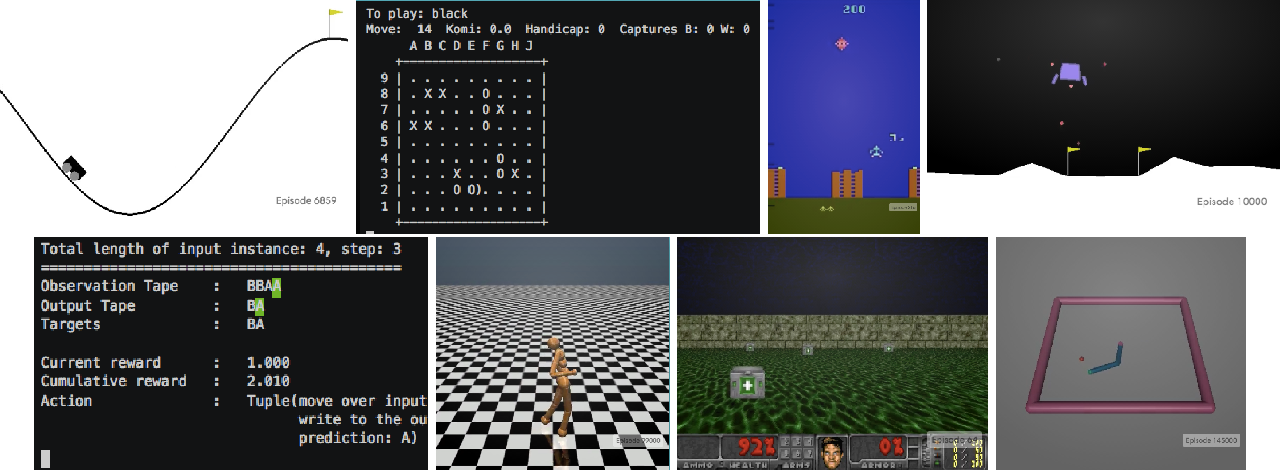
\includegraphics[width=0.7\textwidth]{figures/existing_envs/openai_gym}
				\caption{OpenAI Gym}
				\label{fig:openai_gym}
		\end{subfigure}
		\hfill
		\begin{subfigure}[b]{0.3\textwidth}
				\centering
				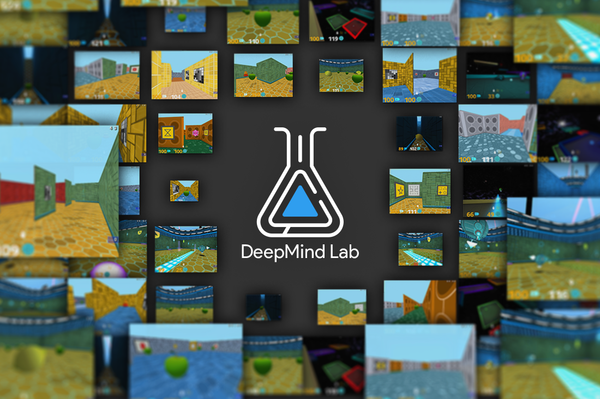
\includegraphics[width=0.7\textwidth]{figures/existing_envs/deepmind_lab.png}
				\caption{DeepMind Lab}
				\label{fig:deepmind_lab}
		\end{subfigure}
		\hfill
		\begin{subfigure}[b]{0.3\textwidth}
				\centering
				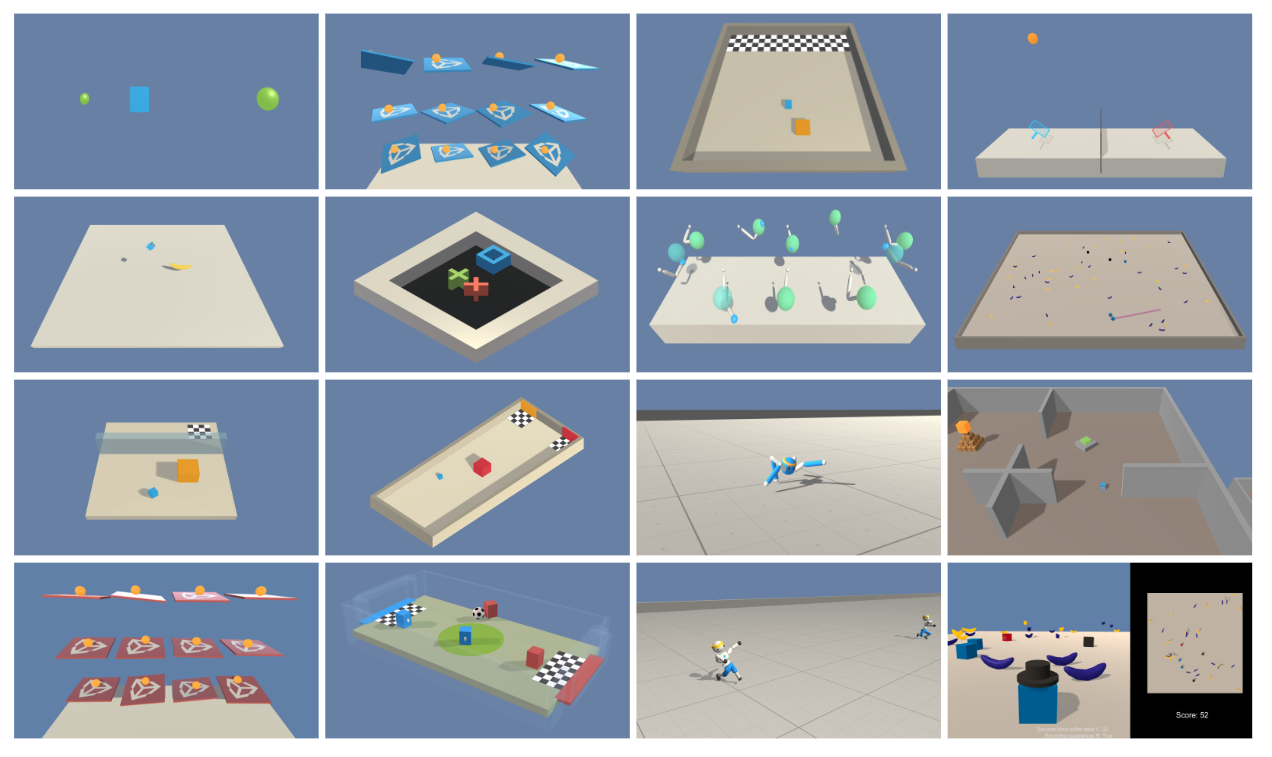
\includegraphics[width=0.7\textwidth]{figures/existing_envs/unity_mlagents.png}
				\caption{Unity MLAgents}
				\label{fig:unity_mlagents}
		\end{subfigure}
		\hfill

		\begin{subfigure}[b]{0.3\textwidth}
				\centering
				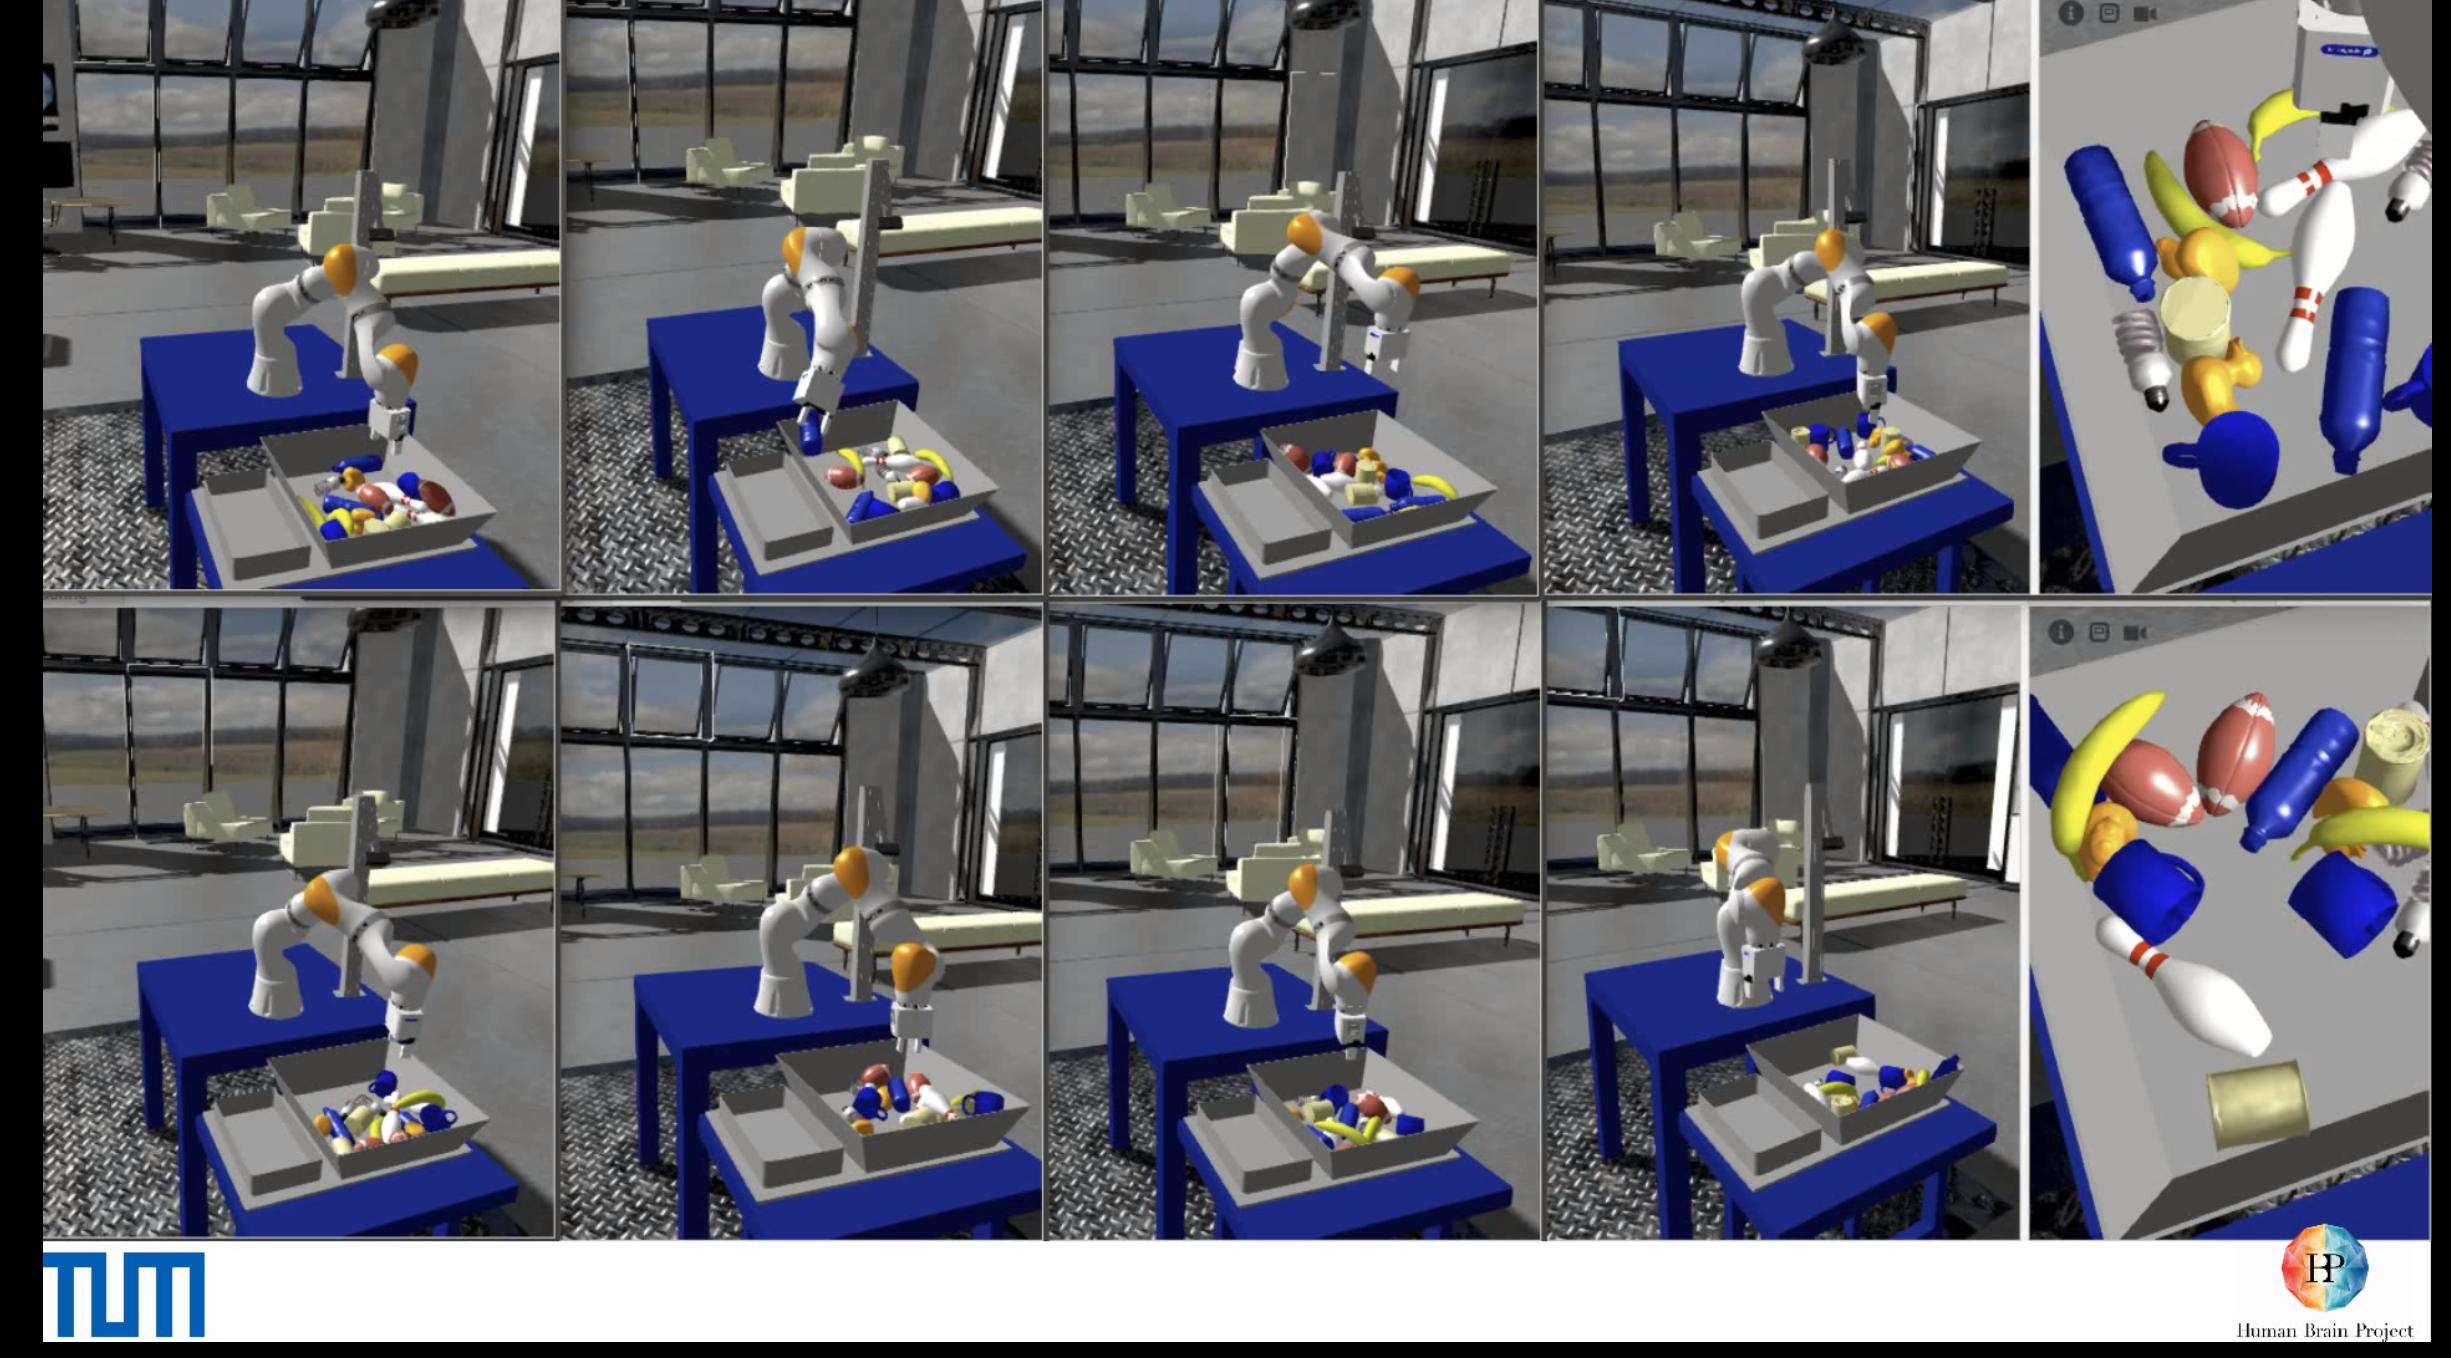
\includegraphics[width=0.7\textwidth]{figures/existing_envs/nrp.png}
				\caption{Neurorobotics Platform}
				\label{fig:atari_2600}
		\end{subfigure}
		\hfill
		\begin{subfigure}[b]{0.3\textwidth}
				\centering
				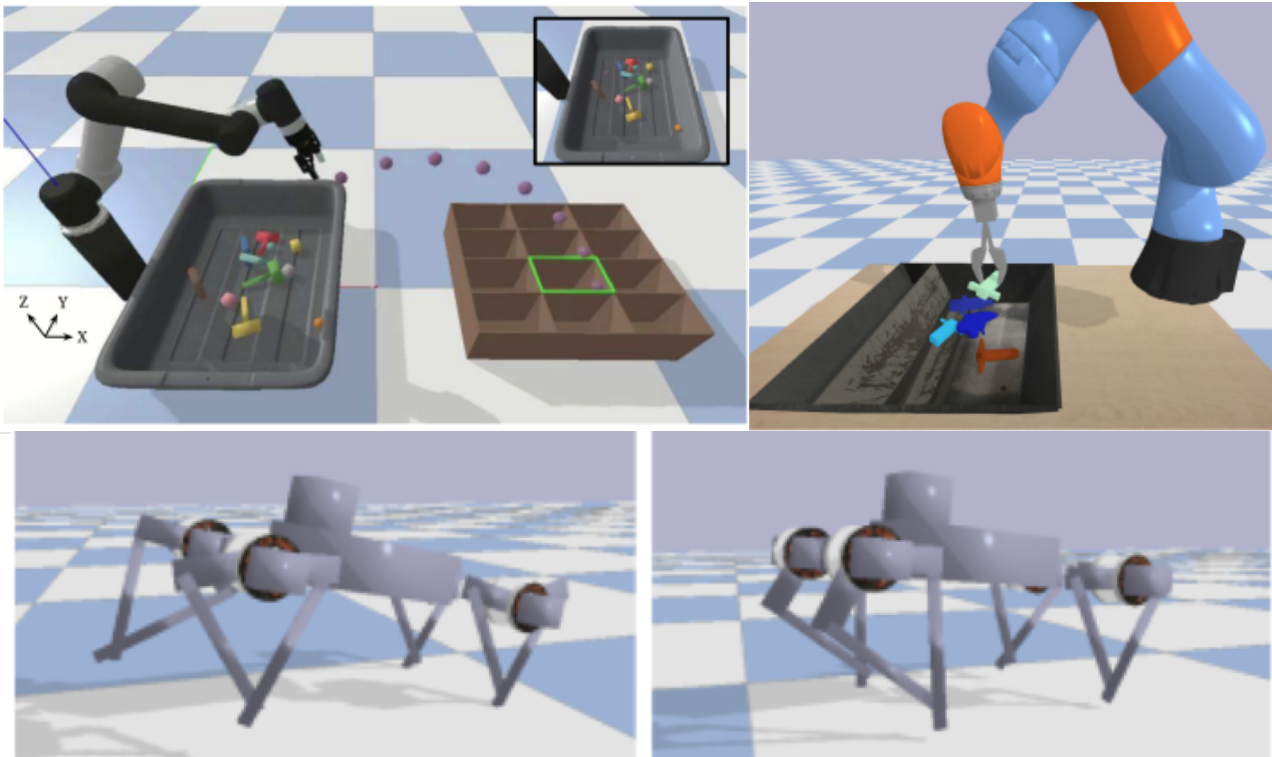
\includegraphics[width=0.7\textwidth]{figures/existing_envs/pybullet.png}
				\caption{PyBullet}
				\label{fig:pybullet}
		\end{subfigure}
		\hfill
		\begin{subfigure}[b]{0.3\textwidth}
				\centering
				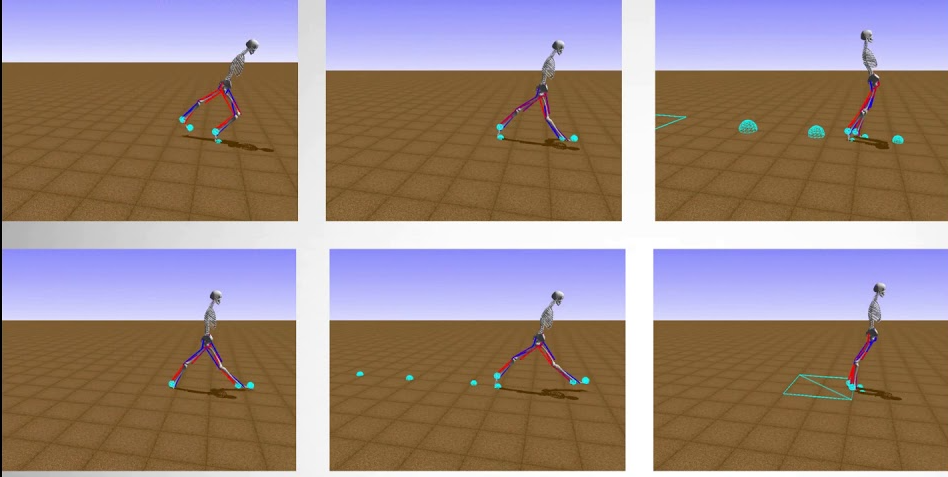
\includegraphics[width=0.7\textwidth]{figures/existing_envs/osim_rl.png}
				\caption{Osim RL: musculoskeletal models in OpenSim}
				\label{fig:osim_rl}
		\end{subfigure}

		\begin{subfigure}[b]{0.3\textwidth}
				\centering
				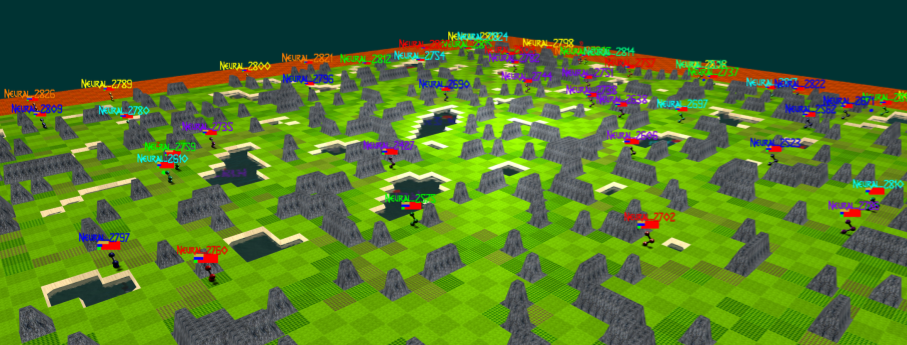
\includegraphics[width=0.7\textwidth]{figures/existing_envs/openai_mmo.png}
				\caption{OpenAI MML}
				\label{fig:openai_mmo}
		\end{subfigure}
		\hfill
		\begin{subfigure}[b]{0.3\textwidth}
				\centering
				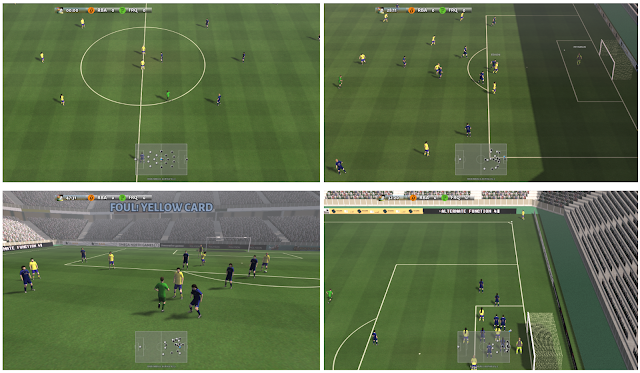
\includegraphics[width=0.7\textwidth]{figures/existing_envs/google_football.png}
				\caption{Google Research Football}
				\label{fig:google_football}
		\end{subfigure}
		\hfill
		\begin{subfigure}[b]{0.3\textwidth}
				\centering
				\includegraphics[width=0.7\textwidth]{figures/existing_envs/deepmind_alphstar.png}
				\caption{StarCraft II Learning Environment}
				\label{fig:deepmind_alphstar}
		\end{subfigure}
	\hfill
		 \caption{Examples of existing Deep RL Environments}
		 \label{fig:envs_examples}
\end{figure}

\clearpage

\subsection{Markov Decision Process}
Formally, reinforcement learning can be described as a Markov decision process, An MDP is a 5-tuple, $ \left\langle S, A, \mathcal{T}, R, \gamma \right\rangle $ which consists of:

\begin{itemize}
		\item A set of all states \(S\), plus a distribution of starting states \(p(s0)\).
		\item A set of valid actions \(A\).
		\item Transition dynamics $ \mathcal{T}\left(\mathbf{s}_{t+1} | \mathbf{s}_{t}, \mathbf{a}_{t}\right) $ that map a state-action pair at time \(t\) onto a distribution of states at time \(t+1\).
		\item An immediate $ \mathcal{R}\left(\mathbf{s}_{t}, \mathbf{a}_{t}, \mathbf{s}_{t+1}\right) $ reward function.
		\item A discount factor \(\gamma \in(0,1)\), where lower values place more emphasis on immediate rewards.
\end{itemize}

Extra objects can be defined depending on problem setting:
\begin{itemize}
		\item $\rho_0$:Initial state distribution
\end{itemize}

Markov Decision Process refers to the fact that the system obeys the \textbf{Markov property}: which indicates that transitions only depend on the most recent state and action, and no prior history, in other words, the future is conditionally independent of the past given the present state. $ p\left(s_{t+1} | s_{1}, a_{1}, \ldots, s_{t}, a_{t}\right)=p\left(s_{t+1} | s_{t}, a_{t}\right) $


\subsection{Rewards and Return}

The reward function \(R\) is critically important in reinforcement learning. It depends on the current state of the world, the action just taken, and the next state of the world:

\begin{center}
		\begin{equation}
				r_{t}=R\left(s_{t}, a_{t}, s_{t+1}\right)
		\end{equation}
\end{center}

The goal of the agent is to maximize some notion of cumulative reward over a trajectory.

There are two kinds of return, \textbf{the finite-horizon undiscounted return}, which is just the sum of rewards obtained in a fixed window of steps:

\begin{center}
		\begin{equation} \label{eq:1}
				R(\tau)=\sum_{t=0}^{T} r_{t}
		\end{equation}
\end{center}

Another kind of return is \textbf{the infinite-horizon discounted return}, which is the sum of all rewards ever obtained by the agent, but \textit{discounted} by how far off in the future they’re obtained. This formulation of reward includes a discount factor \(\gamma \in(0,1)\):

\begin{center}
		\begin{equation} \label{eq:2}
				R(\tau)=\sum_{t=0}^{\infty} \gamma^{t} r_{t}
		\end{equation}
\end{center}

The use of a discount factor is crucial as \textbf{mathematically} an infinite-horizon sum of rewards may not converge to a finite value, and is hard to deal with in equations. But with a discount factor and under reasonable conditions, the infinite sum converges.

\subsection{Policies}
A policy ($\pi$) is a rule used by an agent to decide what actions to take, it's considered as the strategy that the agent employs to determine the next action based on the current state. It maps states to actions $ \pi : \mathcal{S} \rightarrow p(\mathcal{A}=\mathbf{a} | \mathcal{S}) $, the actions that promise the highest reward.

The policy can be deterministic where it is usually denoted by $ \mu: a_{t}=\mu\left(s_{t}\right) $
or stochastic denoted by $ \pi:  a_{t} \sim \pi\left(\cdot | s_{t}\right) $
with the two most common kinds of stochastic policies categorical policies (discrete action spaces) and diagonal Gaussian policies (continuous action spaces).

with two key computations that are very important for training stochastic policies:
\begin{itemize}
		\item sampling actions from the policy,
		\item computing log likelihoods of particular actions, $ \log \pi_{\theta}(a|s) $
\end{itemize}


\subsection{Reinforcement Learning Goal}
The goal of reinforcement learning is to select a policy which maximizes the \textbf{expected return} when the agent acts according to it.

where the \textbf{expected return} denoted by $ J(\pi) $ is:
\begin{center}
		\begin{equation} \label{eq:expected_return}
				J(\pi)=\int_{\tau} P(\tau | \pi) R(\tau)=\underset{\tau \sim \pi}{\mathrm{E}}[R(\tau)]
		\end{equation}
\end{center}

with $ P(\tau | \pi) $ as the probability distributions over T-step trajectories.
\begin{center}
		\begin{equation}
				P(\tau | \pi)=\rho_{0}\left(s_{0}\right) \prod_{t=0}^{T-1} P\left(s_{t+1} | s_{t}, a_{t}\right) \pi\left(a_{t} | s_{t}\right)
		\end{equation}
\end{center}

So the central optimization problem of RL can be described as:
\begin{center}
		\begin{equation}
				\pi^{*}=\arg \max _{\pi} J(\pi)
		\end{equation}
\end{center}
with $\pi^*$ being the optimal policy.


\subsection{Learning optimal policies}
There are two main approaches to solving RL problems: methods based on \textit{value functions} (Critic-only), and methods based on \textit{policy search} (Actor-only).
There is also a hybrid, \textit{actor-critic approach}, which combines both value functions and policy search, where the actor and critic are both represented explicitly and learned separately.
We will now explain these approaches and other useful concepts for solving RL problems.

\subsubsection{Critic-only: Learning based on value functions}
Critic only methods are based on the idea to first find the optimal value function and then to
derive an optimal policy from this value function. 
Value function methods are based on estimating the value (expected return) of being in a given state.
The state-value function $V^{\pi}(\mathbf{s})$ is the expected return when starting in state $\mathbf{s}$ and following $\pi$ henceforth:
\begin{center}
		\begin{equation}
				V^{\pi}(\mathbf{s})=\mathbb{E}[R | \mathbf{s}, \pi]
		\end{equation}
\end{center}

and the optimal state-value function can be defined as
\begin{center}
		\begin{equation}
				V^{*}(\mathbf{s})=\max _{\pi} V^{\pi}(\mathbf{s}) \quad \forall \mathbf{s} \in \mathcal{S}
		\end{equation}
\end{center}

The optimal policy, $\pi^{*}$, has a corresponding state-value function $V^{*}(\mathbf{s})$ where it could be retrieved by choosing among all actions available at $\mathbf{s_t}$ and picking the action $\mathbf{a}$ that maximizes expected optimal value for the succeeding state.

In practice, the MDP is often unknown and the transition dynamics $\mathcal{T}$ are unavailable so the only way to get information about it is by interacting with the environment and observing rewards.
Hence, construct another function, the \textit{state-action value or quality function} $Q^{\pi}(\mathbf{s}, \mathbf{a})$ estimates the value function and derives an optimal policy. 
It is similar to $V^{\pi}$, except that the initial action $\mathbf{a}$ is provided, and $\pi$ is only followed from the succeeding state onwards:
\begin{center}
		\begin{equation}
				Q^{\pi}(\mathbf{s}, \mathbf{a})=\mathbb{E}[R | \mathbf{s}, \mathbf{a}, \pi]
		\end{equation}
\end{center}

A Selection of these approaches \textit{Dynamic programming, Temporal difference learning, 
Eligibility trace} is used in order to learn these functions.
% \clearpage

\subsubsection{Actor-only: Policy search}
Policy search methods do not need to maintain a value function model, but directly search for an optimal policy $\pi^{*}$. This is only possible if the search space is restricted. Typically, a class of policies is parametrized by a real-valued parameters vector $\theta$, these parameters are updated to maximize the expected return $\mathbb{E}[R | \theta]$ using either gradient-based or gradient-free optimization~\parencite{deisenroth2013survey}.

Policy based reinforcement learning is an \textit{optimization} problem, we need to find $\theta$ that maximize the expected return~\eqref{eq:expected_return}.
Some approaches do not use gradient like \textit{Hill climbing, Genetic algorithms}, but the common use is \textit{policy gradients}.


\textbf{Policy Gradients}: Gradients provide a strong learning signal to improve a parameterized policy. In order to compute the expected return \eqref{eq:expected_return}, averaging trajectories generated by the current policy parameterization is needed. This averaging requires either deterministic approximations or stochastic approximations via sampling.
Due to gradients cannot pass through these samples of a stochastic function, 
Hence we use an estimator of the gradient, known in RL as the \textbf{REINFORCE rule}~\parencite{williams1992simple}, \textit{score function}~\parencite{fu2006gradient} or \textit{likelihood-ratio estimator}~\parencite{glynn1990likelihood}.
Gradient ascent using the estimator, which is similar to the practice of optimizing the log-likelihood in supervised learning, increases the log probability of the sampled action, weighted by the return.

\subsubsection{Actor-Critic Method:}
Actor-Critic method is the combination of both \textit{value functions} and an explicit representation of \textit{the policy} as shown in ~\ref{fig:actor_critic}, where The \textit{actor} (policy) learns by using feedback from the \textit{critic} (value function).
These methods trade off variance reduction of policy gradients with bias introduction from value function methods.

\begin{figure}[H]
		\begin{center}
				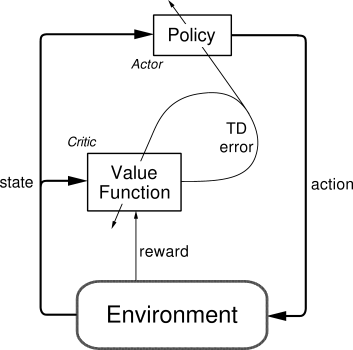
\includegraphics[width=.3\linewidth]{figures/actor_critic.png}
				\caption{Actor-critic set-up. The actor (policy) receives a state from the environment and chooses an action to perform. At the same time, the critic (value function) receives the state and reward resulting from the previous interaction.~\parencite{arulkumaran2017brief}}
				\label{fig:actor_critic}
		\end{center}
\end{figure}


\clearpage

\section{Deep Reinforcement Learning}

Recent breakthrough in deep learning fields relied on efficiently training deep neural network on large training datasets, which improves many fields including \textit{computer vision and speech recognition}. These models are trained directly from raw inputs using stochastic gradient descent to update the networks' weights. These successes lead its way to reinforcement learning in which in connects RL algorithms with deep neural networks to operate directly on raw images and efficiently generate training data using stochastic gradient updates.

\subsection{Overview}
DeepMind\footnote{\url{https://deepmind.com}\label{deepmind}} has lead the way by introduction \textit{\textbf{Deep Q-Network} (DQN)}~\parencite{mnih2015human}, in which the new deep learning model for reinforcement learning, demonstrates its ability to master difficult control policies for Atari 2600 computer games, using only raw pixels as input.

In the following we briefly discuss four state-of-the-art algorithms, \textit{Deep Q Network}, two deep policy search methods: \textit{Deep Deterministic Policy Gradient} and \textit{Proximal Policy Optimization}, also an asynchronous deep actor-critic method called \textit{Asynchronous Advanced Actor-Critic}.
These methods are currently the most popular and effective algorithms, proposed by DeepMind\footref{deepmind} and OpenAI\footnote{\url{https://openai.com}}. In this work, some of these methods are used for experiments.

\subsection{Deep Q Network}
Deep Q Network (\textbf{DQN}) was first proposed by~\parencite{mnih2013playing}, it presents the first deep learning model to successfully learn control policies directly from high-dimensional sensory input using reinforcement learning.

Q-learning algorithm was used to make the decision, using stochastic gradient descent to update the weights. Since deep learning handles only with independent data samples, the \textit{experience replay} mechanism was used to break correlations along with \textit{Fixed Q-target}. DQN algorithm replaces the tabular representation for Q-value function with the deep neural network.

\subsection{Deep Deterministic Policy Gradient}
Since the rise of deep neural network function approximations for learning value or action-value function, deep deterministic policy gradient method have been proposed by~\parencite{lillicrap2015continuous}. It used an \textit{actor-critic} approach based on the \textbf{DPG algorithm}~\parencite{silver2014deterministic}, combined with \textit{experience replay and fixed Q-target} techniques which inspired by \textbf{DQN} to use such function approximation in a stable and robust way. additionally, a robust strategy in deep learning called \textit{batch normalization}~\parencite{ioffe2015batch}is  adopted to scale the range of input vector observations in order to make the network capable of finding hyper-parameters which generalize across environments with different scales of state values.
The problem of exploration in off-policy algorithms like DDPG can be addressed in a very easy way and independently from the learning algorithm. Exploration policy is then constructed by adding noise sampled from a noise process N to the actor policy.

\subsection{Proximal Policy Optimization}
One of the main issue in policy gradient methods is defining the step size (\textit{learning rate $\alpha$}). Hence, the new robust policy gradient methods, which we call Proximal Policy Optimization~\parencite{schulman2017proximal, heess2017emergence} was proposed to solve this problem. It also uses some of the benefits from trust region policy optimization~\parencite{schulman2015trust}. these methods bound parameter updates to a trust region to ensure stability.
This algorithm is similar to natural policy gradient methods and it is also considered as a variant of TRPO, it directly uses the first order optimization methods to optimize the objective.

\subsection{Asynchronous Advanced Actor Critic (\textbf{A3C})}
Asynchronous Advanced Actor Critic~\parencite{mnih2016asynchronous} is an asynchronous method using Advanced Actor-Critic. \textit{\textbf{Asynchronous}} means Asynchronously execute multiple agents in parallel, on multiple instances of the environment and all using a replica of the NN (\textit{asynchronous data parallelism}). It often works in a multi-core CPU or GPU. The idea behind it is that there is a \textit{global network} and \textit{multiple actor-learners} which have their own set of network parameters. A thread is dedicated for each agent, and each thread interacts with its own copy of the environment.
Giving each thread a different exploration policy also improves robustness, since the overall experience available for training becomes more diverse. Moreover, in A3C just one deep neural network is used both for estimation of policy $\pi(s)$ and value function $V_{\pi}(s)$; because we optimize both of these goals together, we learn much faster and effectively. We also don’t need to consider the data correlation and oscillations issues because different agent gets different transitions when playing in the same environments.

\clearpage

\section{Challenges in Reinforcement Learning} 

% TODO:
The two main problems of RL
The highest level description of reinforcement learning is the maximization of some notion of long term return by acting in an environment. There are two fundamental difficulties one encounters while solving RL problems: the balance of exploration vs. exploitation and long term credit assignment.


\textbf{Exploration-vs-exploitation}
Sample inefficiency, reproducibility, and escaping local optima
This is the question every agent must learn to answer from a very early age, do I keep following this policy that’s giving me nice returns, or do I take some relatively sub-optimal actions now in case there’s a possibly bigger payoff later? This problem is so hard because there can be no right answer in general - there is always a trade-off.

Off to a good start.
The famous Bellman update only guarantees convergence to the optimal value function if every state is visited an infinite number of times and every action is tried an infinite number of times in it. So right off the bat, we need an infinite samples to learn, and we need them everywhere!

You may say something like “Why obsess over optimality?”

Fair enough. In most cases, a policy that achieves the goal, doesn’t take too long, and doesn’t mess up too many other things is fine. Sometimes in practice, we are happy to find that a good policy can be learnt in a finite number of steps (20 million is much smaller than infinity). But it is hard to define these subjective notions without attaching numbers to maximize/minimize something. It is even harder to provide any sort of guarantees on it. More on this later.

Ok so let’s just say we are happy with an approximately optimal solution (whatever that means). The number of samples needed to get the same approximation increases exponentially with the state and action space.

But wait, it gets worse.
Without any assumptions, there is no better way to explore than randomly. You can add some heuristics, such as curiosity [2], and they work well in some cases, but we do not have a complete solution yet. After all, you have no reason to believe there’s a bigger or smaller payoff behind any action in a particular state unless you try it.

What’s more, model-free reinforcement learning algorithms typically try to solve the most general formulation of the problem. As in, there are very few assumptions about the form of the state distribution, the transition dynamics of the environment or of optimal policies (for eg. [3])

And this makes sense. Just because you see a great reward once doesn’t mean you will always get it every time you are in that state and take that action. The only sensible thing to do then is to not trust any particular reward too much and only slowly make changes to your belief of how good an action is in a state.

Ok, so you are making small, conservative updates to functions that are trying to approximate expectations of arbitrarily complex probability distributions over an arbitrarily large number of states and actions.

But wait. It actually gets even worse.
Let’s talk about continuous states and actions.

The world at our size seems to be mostly continuous. But that’s a problem for RL. How are you supposed to visit an infinite number of states an infinite number of times and take an infinite number of actions an infinite number of times in them? If only you could generalize some of the knowledge you have learned to unseen states and actions. Supervised learning!!

Exploration in uncertain dynamics also explains why RL seems to be more sensitive to hyper-parameters and random seeds than supervised learning. There are no fixed datasets your networks are training on. The training data is directly dependent on the network output, whatever exploration mechanism you use, and environment randomness. Therefore, with the same algorithm on the same environment in different runs, you may see dramatically different training sets, leading to dramatically different performance (take a look at [4]). Again, the core problem is that of controlling exploration to see similar distributions of states, something that the most general algorithms make no assumptions over.


\textbf{Long term credit assignment}
Reward functions, their design, and transfer
You know how some people will scratch lottery tickets only with a lucky coin because one time they did and they won a lot of money? RL agents are basically playing the lottery at every step and trying to figure out what they did to hit the jackpot. They are maximizing a single number which is the result of actions over multiple time steps mixed in with a good amount of environment randomness. Figuring out which series of actions are actually responsible for the high reward is the problem of credit assignment.

You want rewards to be easy to specify. The promise of reinforcement learning is that you tell a robot when it has done something right and over time it learns how to do that thing reliably. You don’t have to actually know how to do the thing yourself and you don’t have to provide supervision at every step.

The problem actually occurs because the scale at which we can provide rewards for meaningful tasks is much larger than the scale current day algorithms can handle. The robot is operating at a much faster time scale of what joint velocities it should set at every millisecond and the human is expecting to only reward it once it has made a good sandwich. There are many decisions that happen in between and if the gap between the crucial choices and the reward is too big, any current day algorithm will just fail.

There are two solutions to this. One is to reduce the scale at which rewards are provided, i.e. provide shaping rewards more frequently. As usual, though, if you give an optimization algorithm a weakness, it will exploit it all the way to optimality. If the reward is not well designed it can lead to reward hacking.

Ultimately, we fall for this because we forget that the agent is optimizing in the value landscape, not for the immediate rewards. So even if your immediate reward structure seems innocuous, the value landscape may be very non-intuitive and may have many of these exploits if one is not careful.

Which begs the question, why are rewards used in the first place? Rewards are a way of specifying goals that will let us use the power of optimization to get a good policy. Shaping rewards are a way to inject more domain specific knowledge on top.

Are there better ways of specifying goals? In imitation learning, you can slyly sidestep the whole RL problem by asking for labels directly from the target distribution, i.e. the optimal policy. There are other ways of learning without direct rewards [5], or providing goals to agents as images [6]. (Stay tuned for an ICML workshop on Goal Specification in RL!)

Another promising way to deal with long horizons (hugely delayed rewards) is hierarchical reinforcement learning. I was surprised when this did not make it into Alex’s post because it is the most intuitively appealing solution to this problem (but I guess I’m biased!)

Hierarchical RL attempts to decompose a long horizon problem into a series of goals and subgoals. By decomposing the problem, we are effectively dilating the time scale at which decisions are being made. The really exciting stuff is if the policies being learned for subgoals can also be applied to achieving other goals.

The promise is great but we’re not there yet on this either. Most state of the art works only consider hierarchies a single level deep and the goal of transfer to different tasks is hard to achieve.